\documentclass[a4paper,11pt,twocolumn]{article}
\usepackage{lingmacros}
\usepackage{blindtext}
\usepackage{tree-dvips}
\usepackage{amsmath}
\usepackage{multicol}
\usepackage{mathtools}
\usepackage{hyperref}
\usepackage{graphicx}
\graphicspath{ {./Latex/} }

%\pagestyle{headings} Writes the heading on top of the page.
\begin{document}

\title{Regression Analysis of the Franke Function}
\date{2019\\ September}
\author{Eirik Nordgård\\ Geophysical Institute,\ University of Oslo}


\twocolumn[
\begin{@twocolumnfalse}
\maketitle
\begin{abstract}
Ordinary Least Squares, Ridge regression and Lasso regression have been used on data generated by the Franke Function. MSE and R2 score have been evaluated for each model. Ordinary Least Squares seems to be the most accurate regression method on this dataset. Ridge also performs quite well, while the lasso is very dependent on the penalty parameter to provide good results. 
\end{abstract}

All material for this project may be found on 
\url{https://github.com/eirikngard/Project1}

\end{@twocolumnfalse}
]
\

\section{Introduction}

The main aim of this project is to study various linear regression methods in detail. Ordinary Least Squares (OLS), Ridge regression and Lasso regression are the methods which will be investigated. Models using linear regression assumes linear inputs X1, X2,...,Xp. Even though there are many other, no-linear models you might think outperforms the linear models, they actually have a couple of advantages compared to the non-linear models. They are simple to use and provide interpretable descriptions of how the inputs affect the outputs. In situations with small numbers of training cases or if the signal-to-noise ratio is small, linear models can outperform non-linear models in prediction. Also, applying linear methods to transformations of the inputs expands their scope tremendously\cite{Hastie}.
\\
\\
\\
\\

In this project I have used data generated by the Franke function. This is a smooth, terrain-like function with two Gaussian peaks and a small dip often used in interpolation problems.
\begin{figure}[h]
\centering
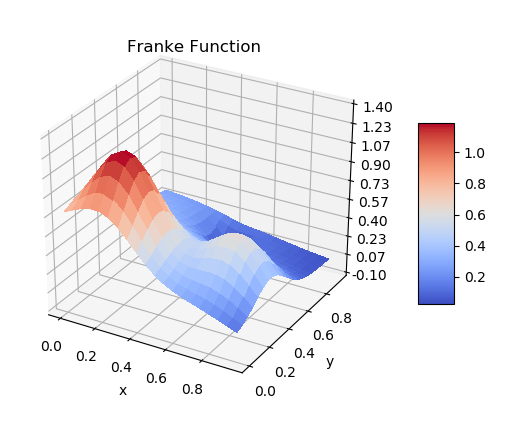
\includegraphics[scale=0.75]{Franke3}
\caption{3D plot of the Franke Function}
\label{Franke3}
\end{figure}
\\
\\
\\

\section{Theory}

\subsection{Linear Regression Models}

The goal is to make a model that predicts a real-valued output $y$ with an input vector $x$. We can make a linear model $y(x_i)$ on the form 
\begin{equation}
\label{e1}
y=\tilde{y}_i+\epsilon_i
\end{equation}

where $\tilde{y}$ is a function of some variable and  
$\epsilon_i\sim{\mathcal{N}}(0,\sigma^2)$ is the normally distributed error with mean, $\mu=0$ and variance = $\sigma^2$. The function $y$ can then be written as 
\begin{equation}
\label{y1}
y=\beta _0 + \sum\limits_{i=1}^n X_j\beta_j+\epsilon_i
\end{equation}

where $\beta$ are unknown coefficients and $X$ is the so called Vandermonde design-matrix with data input vector $X^T=(X_1,X_2,...,X_p)$.

Eq. \eqref{y1} can be rewritten as 
\begin{equation}
y=X\beta+\epsilon
\end{equation}

and thus the approximation can be written as 
\begin{equation}
\tilde{y}=X\beta
\end{equation}
.

To obtain the optimal set of $\beta_i$ a cost function is defined. This function gives a measure of the spread between the exact values $y_i$ and the parametrized values 
$\tilde{y}_i$,

\begin{equation}
C(\beta)=\frac{1}{n}\sum\limits_{i=0}^{n-1}(y_i-\tilde{y}_i)^2
\end{equation}
    
or 
\begin{equation}
\label{c1}
C(\beta)=\frac{1}{n}\lbrace (y-X^T\beta)^T(y-X^T\beta) \rbrace
\end{equation}

in terms of design matrix $X$ and coefficients $\beta$.

To obtain the the optimal set of $\beta$ it is necessary to minimize $C(\beta)$ for all $\beta$. \cite{slides}


\subsubsection{Ordinary Least Squares (OLS)}

%For statistical analysis we usually use a set of training data %$(x_1,y_1)...(x_N,y_N)$ to estimate the $\beta$ parameters. %The most popular estimation method is the least squares method %\textbf{Hastie 44}, where the coefficients $\beta=(\beta_0,\beta_1,...,\beta_p)^T$ are picked to find a linear function X %that minimize the residual sum of squares\footnote{Hastie 45}.

%$$RSS(\beta)=\sum\limits_{i=1}^N(y_i-f(x_i))^2$$
%		  $$=\sum\limits_{i=1}^N(y_i-\beta_0-\sum\limits_{j=1}^p(x_{ij}\beta_j))^2$$
		 
%Furthermore, assuming the training data represent independent %and random draws from the population or if all $y_i$ in the %training data are conditionally independent given the inputs %$x_i$, $RSS(\beta)$ can be rewritten as 

%$$RSS(\beta)=(y-X\beta)^T(y-X\beta)$$

%with the unique solution

%$$\hat{\beta}^{OLS}=(X^TX)^{-1}X^Ty$$	

%Here the hat-rematk indikates this is a predicted value for the true $\beta$. This notation will keep this meaning throughout this text \footnote{Make sure this is the case, dont confuse with ytilde}.

%The solution for beta is the one which minimizes the residuals. 

Solving the minimization problem of \eqref{c1} require 
\begin{equation}
\begin{multlined}
\frac{dC(\beta)}{d\beta_j}= \frac{d}{d\beta}[\frac{1}{n}\sum\limits_{i=0}^{n-1}(y_i-\beta_0x_{i,0}\\-\beta_1x_{i,1}-...-\beta_{n-1}x_{i,n-1})^2] = 0
\end{multlined}
\end{equation}

resulting in 
\begin{equation}
\frac{dC(\beta)}{d\beta}=X^T(y-X\beta)=0
\end{equation}
.

Rewriting this as 
\begin{equation}
X^Ty=X^TX\beta
\end{equation}

gives the solution 
\begin{equation}
\hat{\beta}^{OLS}=(X^TX)^{-1}X^Ty
\end{equation}
	
if the matrix $X^TX$ is invertible.\cite{slides}

Here the hat-rematk indikates this is a predicted value for the true $\beta$. The tilde remark, $\tilde{*}$, has the same meaning. 

To estimate the confidence interval of the $\beta$ obtained by the OLS we need to calculate the variance, $\sigma^2$, of $\hat{\beta}$. Here we must assume uncorrelated observations of $y_i$ and that the variance is constant. Additionally the $x_i$ must be non-random. Derived from equation of $\hat{\beta}$ above we then have\cite{Hastie}
\begin{equation}
Var(\hat{\beta})=(X^TX)^{-1}\sigma ^2 
\end{equation}

where,
\begin{equation}
\label{s1}
\sigma ^2 = \frac{1}{N-p-1} \sum\limits_{i=1}^N (y_i-\hat{y}_i)^2
\end{equation}

$Var(\hat{\beta})$ is called a covariance matrix of the $\beta$ parameter. The denominator in Eq. \eqref{s1} makes it an unbiased estimator of $\sigma^2$. 

The 95\% confidence interval for the $\hat{\beta}$ is 
\begin{equation}
\beta\pm STD*z^{1-\alpha}
\end{equation}


Here $z^{1-\alpha}$ is the 1-$\alpha$ percentile of a normal distribution. $STD$ is the standard deviation of $\beta$, or the diagonal elements of $(X^TX)^{-1}$. For the 95\% confidence interval we have $\alpha =0,025$ and $z^{1-0,025}=1,96$\cite{Hastie}.  

A visualization of how far off the ols method is, is displayed in Fig.\ref{olsdeviation}.
\begin{figure}[h]
\centering
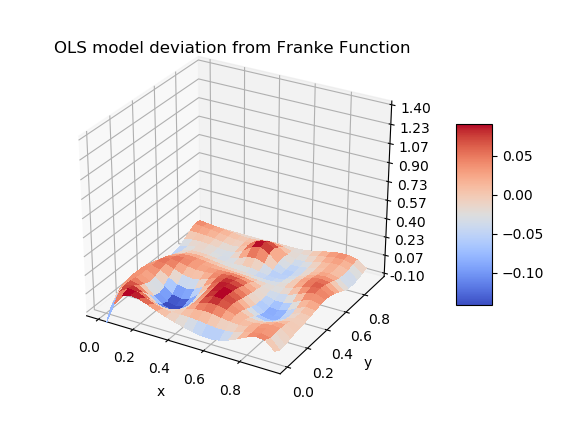
\includegraphics[scale=0.75]{olsdeviation}
\caption{OLS deviation from the Franke Function}
\label{olsdeviation}
\end{figure}

\subsubsection{RIDGE Regression}

Ridge regression is a shrinkage method very similar to OLS. The goal of ridge regression is to shrink the regression coefficients. This is done by imposing a penalty on their size, minimizing the penalized residual sum of squares. The penalty, $\lambda$, is often called a hyper-parameter. Large value of $\lambda$ results in large amount of shrinkage. The ridge shrinking problem can be written as
\begin{equation}
\begin{multlined}
\hat{\beta}^{RIDGE}=\underset{\beta}{argmin}\lbrace\sum\limits_{i=1}^N(y_i-\beta_0\\-\sum\limits_{j=1}^px_{ij}\beta_j)^2+\lambda\sum\limits_{j=1}^p\beta_j^2\rbrace
\end{multlined}
\end{equation}

with solution 
\begin{equation}
\beta^{RIDGE}=(X^T X + \lambda I)^{-1} X^T y
\end{equation}

Here $I$ is the $pxp$ identity matrix. 

A visualization of how far off the ridge method is, is displayed in Fig.\ref{ridgedeviation}.
\begin{figure}[h]
\centering
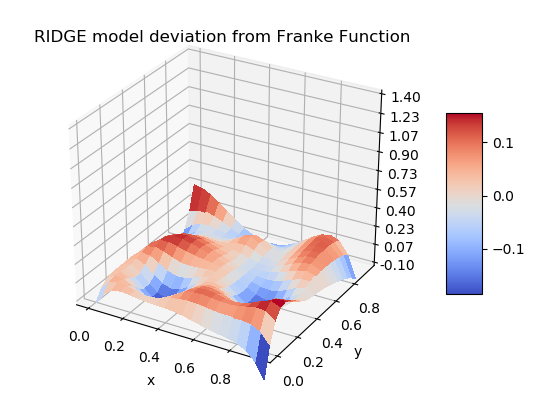
\includegraphics[scale=0.75]{ridgedeviation}
\caption{RIDGE deviation from the Franke Function}
\label{ridgedeviation}
\end{figure}

\subsubsection{LASSO Regression}

Like ridge regression, the lasso is a shrinkage method.
The lasso shrinkage problem in its Lagrangian form can be written 
\begin{equation}
\begin{multlined}
\hat{\beta}^{LASSO}=\underset{\beta}{argmin}\lbrace\frac{1}{2}\sum\limits_{i=1}^N(y_i-\beta_0\\-\sum\limits_{j=1}^px_{ij}\beta_j)^2+\lambda\sum\limits_{j=1}^p\mid\beta_j\mid\rbrace
\end{multlined}
\end{equation}

which is different from the ridge problem only in the penalty $\sum\mid\beta_j\mid$. Since this term makes the solution for $\beta$ nonlinear in $y_i$, there are no definite expression for the solution as in the ridge regression. The solution is obtained by solving a programming problem using the functionalities in the scikit-learn library. Similarly to the ridge method, the penalty parameter $\lambda$ must be chosen to minimize the expected prediction error for the problem. The difference from ridge is that in stead of doing a proportional shrinkage, each $\beta$ is shrunk by a constant penalty parameter $\lambda$\cite{Hastie} 

A visualization of how far off the lasso method is, is displayed in Fig.\ref{lassodeviation}.
\begin{figure}[h]
\centering
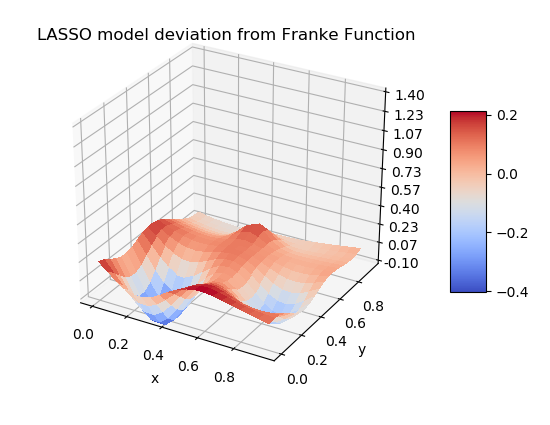
\includegraphics[scale=0.75]{lassodeviation}
\caption{LASSO deviation from the Franke Function}
\label{lassodeviation}
\end{figure}

\subsubsection{Cross-Validation}

When creating a model you want to estimate the prediction error (performance) of the model. To test the prediction performance we spit the data into two sets, a training set and a test set. The training set plays the role of the original data which the model it self is built upon, while the test data is novel data which is used to evaluate the prediction performance of the model. This splitting procedure can be done for a collection of penalty parameter choices, $\lambda$. Performing the splitting many times allows us to pick the $\lambda$ that yields the model with the best prediction performance on average. Additionally we would like to set aside a validation set to evaluate the predictive performance of our model. This set is picked to allow the model to test on data it has not seen before.\cite{slides} $K-fold cross validation$ is one method that handles this problem, since data sets are normally too small to allow us to set aside a validation set. Another problem arising when doing this repetitive splitting is that some data samples may end up in a vast majority of the splits in the training or test sets. This may influence the prediction evaluation. K-fold is one method that handles this by structuring the data splitting.\cite{Hastie}\cite{slides}


\subsubsection{\textit{k}-fold Cross-Validation}
 
The data are divided into \textit{k} more or less equally sized, exclusive subsets. For each split, one of the subsets acts as the test set while all the remaining subsets acts as the training set. This is repeated $\textit{k}-1$ times for many splits. Such splitting results in a balanced representation of the data points in both training and test set for all the splits. Still the division into the \textit{k} subsets involves some degree of randomness, which may be fully excluded when choosing \textit{k}=\textit{n}. This particular case is referred to as leave-one-out cross-validation. 

\subsubsection{Bootstrap}

The bootstrap is used for assessing statistical accuracy. The aim of the bootstrap is thus to estimate the expected prediction error $Err$. After splitting the data into a training and a test set, the basic idea is to randomly draw datasets with replacement from the training data with same size as the original training set. This is repeated $\textit{B}$ times (for instance 100 or 1000), giving $\textit{B}$ datasets. For each of these bootstraps we refit the model and evaluate the fits over the replications.\cite{Hastie}  


\subsubsection{Bias-Variance Tradeoff}

The cost function 
\begin{equation}
C(X,\beta)=\frac{1}{n}\sum\limits_{i=0}^{n-1}(y_i-\tilde{y})^2=E[(y-\tilde{y})^2]
\end{equation}

can be rewritten as 
\begin{equation}
\begin{multlined}
E[(y-\tilde{y})^2]=\frac{1}{n}\sum\limits_i(f_i-E[\tilde{y}])^2+\\ \frac{1}{n}\sum\limits_t(\tilde{y}_i-E[\tilde{y}])^2+\sigma^2
\end{multlined}
\end{equation}

When creating a predictive model it is important to consider the prediction errors such as variance and bias of the model. What we call the bias-variance tradeoff is problem of minimizing both the bias and the variance at the same time. The bias is the difference the average prediction of the model and the true value which the model is trying to predict. High bias corresponds to a oversimplification of the model, thus underfitting the data. This can often lead to high errors on training and test data. 

\begin{equation}
Bias=\frac{1}{n}\sum\limits_{i}^{}(y_i-\tilde{\hat{y}})^2
\end{equation}
  
The variance is the variability of the model prediction for a given data point which indicated the spread of the data. High variance is often a result of overfitting, which means that the model captures too much of the noise along with the underlying datapattern. Thus, models with high variance does not generalize on the data it has not yet seen. 

The objective is to find  function $\hat{f}(x)$, denoted $\hat{f}$, that in the best possible way approximates some true function $f(x)$, denoted $f$. \textit{The best way possible} is made by minimizing the MSE for $y$ and $\hat{f}(x)$ for all $x$.\cite{wiki} 
For any function $\hat{f}$ we can decompose the expected error like this:
\begin{equation}
E[(y-\hat{f}(x))^2]=Bias[\hat{f}(x)])^2+Var[\hat{f}(x)]+\sigma^2
\end{equation}

where 
\begin{equation}
Bias[\hat{f}(x)]=E[\hat{f}(x)]-E[f(x)]
\end{equation}

and 
\begin{equation}
Var[\hat{f}(x)]=E[\hat{f}(x)^2] - E[\hat{f}(x)]^2
\end{equation}

Since $\epsilon$ and $\hat{f}$ are independent,

\begin{equation}
E[(y-\hat{f})^2]=E[(f+\epsilon-\hat{f})^2]
\end{equation}

we have
\begin{equation}
\label{b1}
=Bias[\hat{f}]^2+\sigma^2+Var[\hat{f}]
\end{equation}

See full derivation\cite{wiki} in the Appendix.  


We can rewrite Eq. \eqref{b1} to 

\begin{equation}
\label{b2}
\begin{multlined}
E_{rr}(x)=Bias^2+Variance\\+Irreducibleerror
\end{multlined}
\end{equation}


The bias term in Eq. \eqref{b2} is the squared difference between the true mean and the expected value of the estimate. As the complexity $k$ of a model increases, the bias will most likely also increase. The variance term will decrease as the inverse of $k$. The last term is the variance of the irreducible error. This is simply a measure of noise in our the data which is always present and therefore unavoidable.  

The bias-variance tradeoff is therefore about balancing the bias and the variance to a point where they both are acceptable, where the test error is at a minimum. Too high model complexity results in high variance, whereas too low complexity results in too high bias and vice versa.\cite{Hastie}


The more complex our model $\hat{f}(x)$ is, the more data points it will capture, and the lower the bias will be. However, complexity will make the model "move" more to capture the data points, and hence its variance will be larger\cite{wiki}.

\section{Method}

Defining the Franke function is done using the code provided in in the Project1 PDF (\url{https://github.com/CompPhysics/MachineLearning/tree/master/doc/Projects/2019/Project1}).

First off I have defined the basic functions MSE, R2 score, bias and variance defined in the regression slide\cite{slides}. These functions have input $(data,model)$ and returns the current value. The confidence interval of the $\beta$ is also calculated in this manner. 

For the regression, the design matrix $X$ is needed. This is calculated using x and y flattened creating rows $[1, x, y, x^2, xy, xy^2, etc.]$ depending on the argument n, polynomial degree I want to fit. In the regression itself, this matrix is used to calculate the $\beta$ values, using matrix-inversions. 
With z beeing the data provided by the Franke Function, this line may look like this:
$$Beta_{ols}=$$
$$np.linalg.inv(X.T.dot(X)).dot(X.T).dot(z)$$
Here, \textit{np} is used to access the \textit{NumPy} library functionality. More information on the \textit{NumPy} functionalities can be found on \url{https://numpy.org}. Thereafter, the prediction is calculated using the $\beta$s and the desig matrix $X$. This procedure is repeated for ridge regression as well, but due to an inversion problem the \textit{scikit-learn} functionality is used to perform the lasso regression. More information on \textit{scikit-learn} can be found on \url{https://scikit-learn.org/stable/}. For comparison on the ols and ridge I halve also calculated the MSE using \textit{scikit-learn} as well.

For a simple resample I used \textit{train\_test\_split}, giving an overview of the model performance. Typically this gives results like this:

$$The\:model\:performance\:for\:training\:set$$
$$------------------$$
$$MSE(scikit ols)\: is\quad 0.00225729$$
$$MSE(ols)\: is\quad 0.00225729$$
$$MSE(ridge)\: is\quad 0.03072305$$
$$MSE(lasso)\: is\quad  0.02490839$$
$$R2\:(ols)\: is\quad0.97134498$$

and

$$The\:model\:performance\:for\:testing\:set$$
$$------------------$$
$$MSE(scikit\:ols) is\quad 0.00207010$$
$$MSE (ols)\: is\quad 0.00130538$$
$$MSE (ridge)\:is\quad0.01264897$$
$$MSE (lasso)\:is\quad0.02770861$$
$$R2\: score\: is \quad0.97791144$$

Tuning the penalty parameter to get the best MSE is done using two foor-loops. One creating the design matrix looping over the polynomial degree from 1 to 5. Inside this I loop over a logarithmic $\lambda$-scale, calculating MSE and R2 score using ridge regression.


\section{Results}

To find the optimal $\lambda$ value for the ridge regression it was necessary to manually tune parameter to find the lowest MSE possible. For Ridge regression, the MSE calculated by my own regression code seamed to explode at $\lambda$ around $10^{-1}$ in Fig.\ref{mselamb}
\begin{figure}[h]
\centering
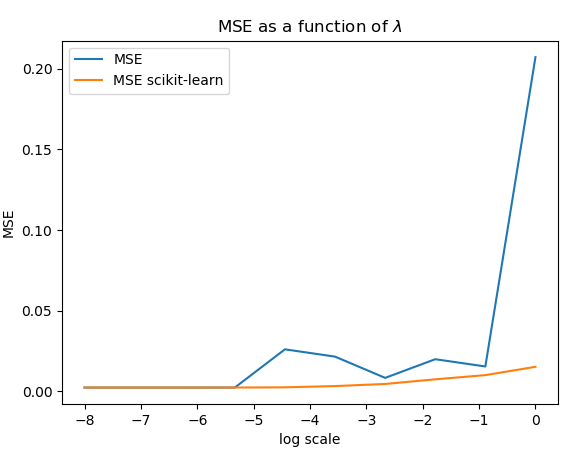
\includegraphics[scale=0.75]{mselam}
\caption{MSE plotted as function of $\lambda$. The x-axis is logarithmic, where $-1$ corresponds to $10^{-1}$}
\label{mselamb}
\end{figure}
For comparison, the MSE calculated by scikit-learn is also showing a slight increase towards higher values of $\lambda$, but does not spike like my code. The overall optimal parameter is around $10^{-5.3}$, providing a MSE of 0.00220566. Additionally, two local lows exist around $10^{-2.7}$ and $10^{-0.9}$, also providing very low MSE (a number). 
Equivalently, Fig.\ref{r2lamb} shows R2 score for the ridge regression is very good (very close to 1) at these $\lambda$ as well.
For larger values of $\lambda$ the MSE spikes through the roof, possibly indicating a numerical instability at certain points. To better display the optimal MSE for my model I would ideally create a heatmap, but due to this problem giving very large MSE this was not possible. 

\begin{figure}[h]
\centering
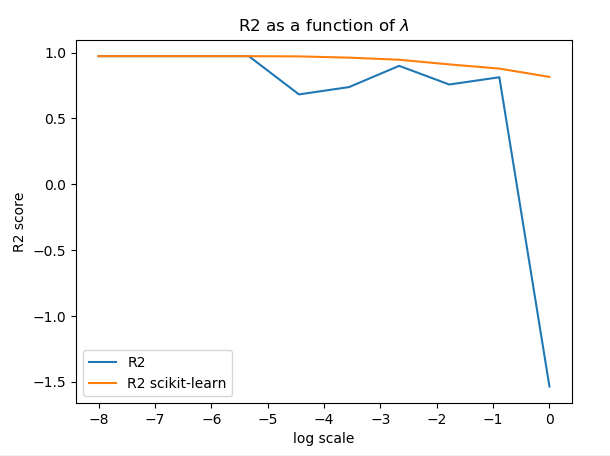
\includegraphics[scale=0.75]{r2lam}
\caption{R2 score plotted as function of $\lambda$}
\label{r2lamb}
\end{figure}

From the regression results it is clear that the OLS provides the lowest MSE of the three methods on the Franke function without noise. This result also hold for the R2 score. The difference in bias for the three methods are marginal. This result is expected (why) since the Franke function is a smooth function. Adding noise rapidly increases the MSE for all three methods. Also the R2 becomes closer and closer to zero.

In Fig.\ref{lamlow} the ridge regression performs slightly worse than the OLS with $\lambda$ around order $10^{-4}$. This also holds for higher values of $\lambda$. The smaller the penalty parameter, the closer the lasso comes to the ridge and OLS. As displayed in Fig. \ref{lamlow}, lasso i performing fairly well compared to ridge and OLS, but once the penalty parameter increases it performs very bad, see Fig.\ref{lamhigh}.The lasso drives the coefficients to zero for small values of $\lambda$.

\begin{figure}[h]
\centering
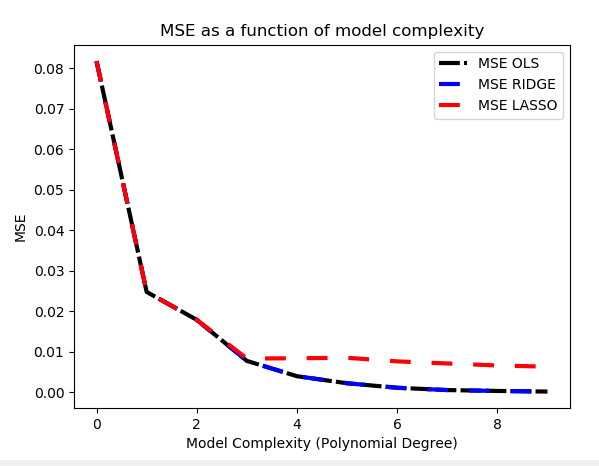
\includegraphics[scale=0.75]{msecomp_lam0001}
\caption{MSE as function of model complexity. $\lambda=0.0001$}
\label{lamlow}
\end{figure}

\begin{figure}[h]
\centering
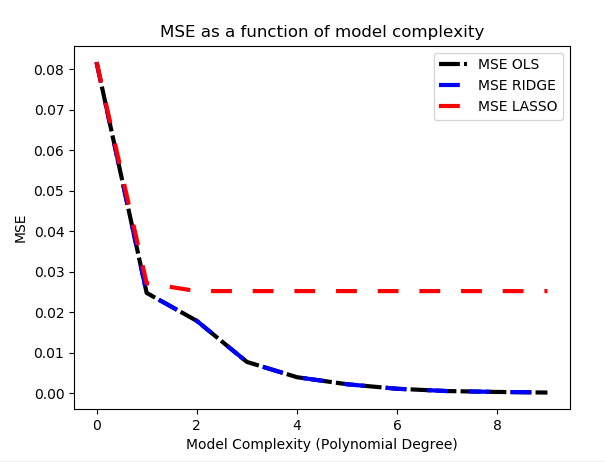
\includegraphics[scale=0.75]{msecomp_lam01}
\caption{MSE as function of model complexity. $\lambda=0.01$}
\label{lamhigh}
\end{figure}

Using the $train\_test\_split$ function provided by scikit-learn the model performance was tested for both the training set and the test set of the data. 

The confidence intervals of the $\beta$ was calculated for each of the regression methods, resulting in the plots in Fig. \ref{confols} to Fig.\ref{conflasso}.

\begin{figure}[h]
\centering
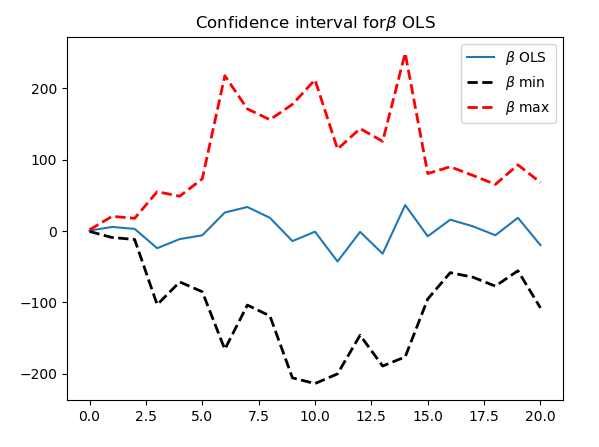
\includegraphics[scale=0.75]{confols}
\caption{Confidence interval for $\beta_{OLS}$}
\label{confols}
\end{figure}

\begin{figure}[h]
\centering
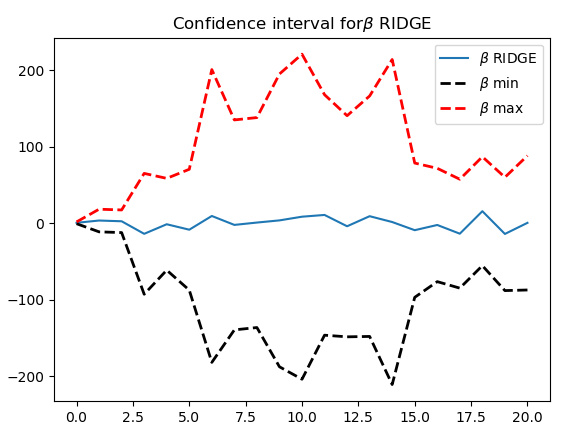
\includegraphics[scale=0.75]{confridge}
\caption{Confidence interval for $\beta_{RIDGE}$, $\lambda=0.01$}.
\label{confridge}
\end{figure}

\begin{figure}[h]
\centering
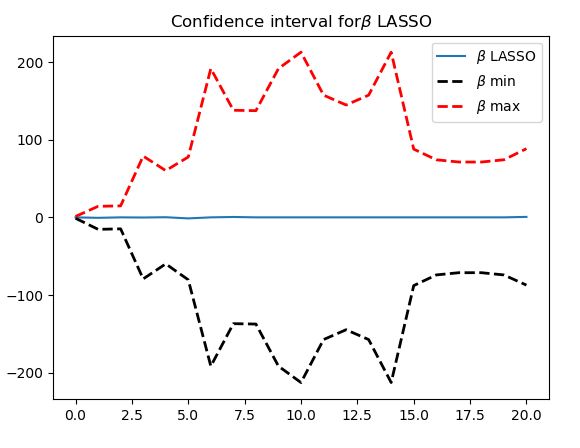
\includegraphics[scale=0.75]{conflasso}
\caption{Confidence interval for $\beta_{LASSO}$, $\lambda=0.001$}.
\label{conflasso}
\end{figure}


\section{Conclusion}

Ordinary Least Squares seems to be the most accurate regression method on the data provided by the Franke Function. The MSE computed by the ols i very low, and you are not in need of tuning a penalty parameter as in ridge or lasso. Ridge also performs quite well for given penalty parameters $\lambda$,  while the lasso is very dependent on the penalty parameter to provide good results. For small $\lambda$ the lasso performs quite good, although the performance weakens rapidly for increasing $\lambda$. 
\\
As stated in the project description, this analysis should also have been done on a real terrain data set. The result of doing so would most likely not have been as clear as for the Franke data. 

\section{Appendix}

Derivation of the bias-variance tradeoff \cite{wiki}. 
$$E[(y-\hat{f})^2]=E[(f+\epsilon-\hat{f})^2]$$
$$=E[(f+\epsilon-\hat{f}+E[\hat{f}]-E[\hat{f})^2]$$
$$=E[(f-E[\hat{f}])^2]+E[\epsilon^2]+E[E[\hat{f}-$$
$$\hat{f})^2]+2E[(f-E[\hat{f}])\epsilon]+2E[\epsilon(E[\hat{f}]$$ $$-\hat{f})]+2E[(E[\hat{f}]-\hat{f})(f-E[\hat{f}])]$$
$$=(f-E[\hat{f}])^2+E[\epsilon^2]+E[(E[\hat{f}]-\hat{f})^2]$$   $$+2(f-E[\hat{f}])E[\epsilon]$$
$$+2E[\epsilon]E[E[\hat{f}]-\hat{f}]$$
$$+2E[E[\hat{f}]-\hat{f}](f-E[\hat{f}])$$
$$=(f-E[\hat{f}])^2+E[\epsilon^2]+E[E[\hat{f}-\hat{f})^2]$$
$$=(f-E[\hat{f}])^2+Var[y]+Var[\hat{f}]$$
$$=Bias[\hat{f}]^2+Var[y]+Var[\hat{f}]$$
$$=Bias[\hat{f}]^2+\sigma^2+Var[\hat{f}]\cite{wiki}$$

\
Bootstrap and \textit{k}-fold cross validation calculations using Mortens code.

\begin{figure}[h]
\centering
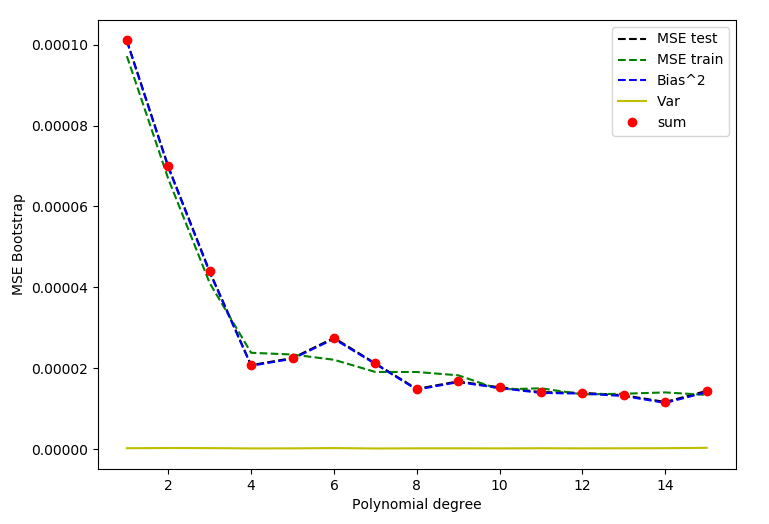
\includegraphics[scale=0.75]{msebootstrap}
\caption{MSE for test and train set, bias and variance calculated using bootstrap.}
\label{msebootstrap}
\end{figure}

\begin{figure}[h]
\centering
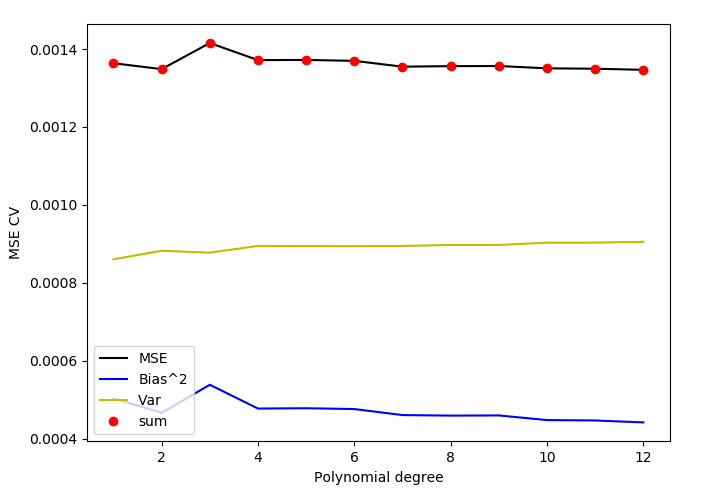
\includegraphics[scale=0.75]{msekfold}
\caption{MSE for test and train set, bias and variance calculated using \textit{k}-fold cross validation}
\label{conflasso}
\end{figure} 

\twocolumn
[
\begin{@twocolumnfalse}


\section{References}
Give always references to material you base your work on, either scientific articles/reports or books.
Refer to articles as: name(s) of author(s), journal, volume (boldfaced), page and year in parenthesis.
Refer to books as: name(s) of author(s), title of book, publisher, place and year, eventual page numbers

\medskip

\begin{thebibliography}{9}
\bibitem{Hastie}
Hastie, Trevor. Tibshirani, Robert. Friedman, Jerome.
\textit{The Elements of Statistical Learning}.
\textit{Data Mining, Interference, and Prediction}.
Second Edition.
Springer, 2009.
Chapter 3, Chapter 7

\bibitem{slides}
M. Hjorth-Jensen
Lecture Notes in FYS-STK4155. \textit{Data Analysis and Machine Learning: Linear Regression and more Advanced Regression Analysis.}
URL:
https://compphysics.github.io/MachineLearning/doc/pub/Regression/html/Regression.html  
Unpublished, 2019. 
 
\bibitem{wiki}
Wikipedia: Bias-Variance tradeoff
URL:
\url{https://en.wikipedia.org/wiki/Bias–variance_tradeoff}
Read: 23.09.2019
 
\end{thebibliography} 

\end{@twocolumnfalse}
]
%\end{multicols}

\end{document}